\documentclass[11pt]{beamer}

\usepackage[utf8]{inputenc}
\usepackage{xcolor}
\usepackage{caption}
\usepackage[natbibapa]{apacite}
\usepackage{bbm}
\bibliographystyle{apacite}
\renewcommand{\bibsection}{\subsubsection*{\bibname}}
\renewcommand*{\bibfont}{\scriptsize}

\usepackage{pgfplots}
\usepackage{tikz}

\pgfplotsset{compat=1.16}


\usetheme{Ilmenau}
\usecolortheme{lily}
\newcommand{\light}[2][35]{\color{fg!#1}#2}

\DeclareMathOperator*{\argmin}{arg\,min}

% Nicer looking Itemize and enumerate environments
\newenvironment{wideitemize}{\itemize\addtolength{\itemsep}{14pt}}{\enditemize}
\newenvironment{wideenumerate}{\enumerate\addtolength{\itemsep}{14pt}}{\endenumerate}


\defbeamertemplate*{footline}{myminiframes theme}
  {%
    \begin{beamercolorbox}[colsep=1.5pt]{upper separation line foot}
    \end{beamercolorbox}
    \begin{beamercolorbox}[ht=2.5ex,dp=1.125ex,%
      leftskip=.3cm,rightskip=.3cm plus1fil]{author in head/foot}%
      \leavevmode{\usebeamerfont{author in head/foot}\insertshortauthor}%
      \hfill%
      {\usebeamerfont{institute in head/foot}\usebeamercolor[fg]{institute in head/foot}\insertshortinstitute}%
    \end{beamercolorbox}%
    \begin{beamercolorbox}[ht=2.5ex,dp=1.125ex,%
      leftskip=.3cm,rightskip=.3cm plus1fil]{title in head/foot}%
      {\usebeamerfont{title in head/foot}\insertshorttitle\hfill \insertframenumber/\inserttotalframenumber}%<-here
    \end{beamercolorbox}%
    \begin{beamercolorbox}[colsep=1.5pt]{lower separation line foot}
    \end{beamercolorbox}
}





\title{From Value Added to Welfare Added: A Social Planner Approach to Education Policy and Statistics}
\author{
Tanner S Eastmond\inst{1} \and Nathan Mather\inst{2} \and Michael Ricks\inst{3}} 
\date{\vspace{-8ex}}
\institute[]{\inst{1}Department of Economics, University of California San Diego, \and \inst{2}Department of Economics, University of Michigan}
\date{}

\begin{document}




%%%%%%%%%%%%%%%%%%%%%%%%%%%%%%%%%%%%%%%%%%%%%%%%%%%%%%%%
%%%%%%%%%%%%%%%%%%%%%% Tile Page. %%%%%%%%%%%%%%%%%%%%%%
%%%%%%%%%%%%%%%%%%%%%%%%%%%%%%%%%%%%%%%%%%%%%%%%%%%%%%%%

\begin{frame}
    \maketitle
\end{frame}




%%%%%%%%%%%%%%%%%%%%%%%%%%%%%%%%%%%%%%%%%%%%%%%%%%%%%%%%
%%%%%%%%%%%%%%%%%%%%% Introduction %%%%%%%%%%%%%%%%%%%%%
%%%%%%%%%%%%%%%%%%%%%%%%%%%%%%%%%%%%%%%%%%%%%%%%%%%%%%%%

\section{Introduction}

%%%%%%%%%%%%%%%%%%%%%%%%%%%%%%%%%%%%%%%%%%%%%%%%%%%%%%%%
%%%%%%%%%%%%%%%%%%%%%%%%%%%%%%%%%%%%%%%%%%%%%%%%%%%%%%%%

\begin{frame}{Value Added Measures: The Goal}
\begin{wideitemize}
    \item Value added measures (VAM) identify the most and least effective teachers
    \item We know teachers respond to incentives
    \begin{itemize}
        \item {\color{gray}{\citep{jacob2003rotten, neal2010left, pope2019effect}}}
    \end{itemize}
    \item We know VAM capture something real
    \begin{itemize}
        \item {\color{gray}{\citep{chetty2014measuring2, pope2017multidimensional}}}
    \end{itemize}
    \item We know there is heterogeneity VAM do not catch
    \begin{itemize}
        \item {\color{gray}{\citep{ehrenberg1995teachers, dee2005teacher, lockwood2009}}}
    \end{itemize}
\end{wideitemize}

\end{frame}


%%%%%%%%%%%%%%%%%%%%%%%%%%%%%%%%%%%%%%%%%%%%%%%%%%%%%%%%
%%%%%%%%%%%%%%%%%%%%%%%%%%%%%%%%%%%%%%%%%%%%%%%%%%%%%%%%

\begin{frame}{Value Added Measures: A Policy Disconnect  }
\begin{wideitemize}

    \item Disconnect between VAM and education policy such as No Child Left Behind
    \begin{itemize}
        \item VAM are mean-oriented statistics: a teachers average impact on students' scores
        \item Carries \textbf{implicit normative} welfare weights 
    \end{itemize}
    
    \item  We propose a set of more flexible heterogeneous VAM 
    \begin{itemize}
        \item Assess teachers' heterogeneous impacts
        \item  Weight effects according to an \textbf{explicit normative} policy goal or welfare criterion
    \end{itemize}


\end{wideitemize}

\end{frame}


%%%%%%%%%%%%%%%%%%%%%%%%%%%%%%%%%%%%%%%%%%%%%%%%%%%%%%%%
%%%%%%%%%%%%%%%%%%%%%%%%%%%%%%%%%%%%%%%%%%%%%%%%%%%%%%%%

\begin{frame}{Research Goals}

\begin{wideenumerate}
     \item Build a welfare-relevant framework for VAM (and other educational statistics) 
     \begin{itemize}
         \item Can we accommodate any policy or normative goal?
     \end{itemize}
    \item Estimate VA heterogeneity along the achievement distribution
    \begin{itemize}
        \item Do certain teachers excel at teaching certain students? 
    \end{itemize}
    \item Simulate data to test new methods
    \begin{itemize}
        \item Are these methods feasible? Accurate? Informative? 
    \end{itemize}
    \item Employ methods in real data
    \begin{itemize}
        \item What implications do rank inversions have for welfare?
        \item What implications are there for possible policies?
    \end{itemize}  

\end{wideenumerate}
\end{frame}




%%%%%%%%%%%%%%%%%%%%%%%%%%%%%%%%%%%%%%%%%%%%%%%%%%%%%%%%
%%%%%%%%%%%%%%%%%%%%%%%% Methods %%%%%%%%%%%%%%%%%%%%%%%
%%%%%%%%%%%%%%%%%%%%%%%%%%%%%%%%%%%%%%%%%%%%%%%%%%%%%%%%

\section{Methods}

%%%%%%%%%%%%%%%%%%%%%%%%%%%%%%%%%%%%%%%%%%%%%%%%%%%%%%%%
%%%%%%%%%%%%%%%%%%%%%%%%%%%%%%%%%%%%%%%%%%%%%%%%%%%%%%%%

\begin{frame}{Estimating Standard  Value Added}

\begin{wideitemize}
    \item In theory test scores are a function of testing ability, value added, and noise
    \begin{align*}
    y_{ijt}  &= a_{it} + \epsilon_{ijt} \\
    y_{ijt}  &= a_{it-1} + VA_j(a_{it-1}) + \epsilon_{ijt}
    \end{align*}
 
    \item We don't observe testing ability. Traditional VAM assumptions:
    \begin{itemize}
        \item Predict testing ability with characteristics (including lagged scores): $X_{it}$
        \item Assume homogeneity within and across teachers $VA_j(\cdot)=\gamma_j$ with no $ij$ error
    \end{itemize}
    \begin{align*}
    y_{ijt}  &= \beta X_{it} +\Gamma D_{it} +\mu_{jt} + \eta_{it}
    \end{align*}
    
    \item Note the $\mu_{jt}$ variation could pick up $ij$ variation.
       
    
\end{wideitemize}
\end{frame}


%%%%%%%%%%%%%%%%%%%%%%%%%%%%%%%%%%%%%%%%%%%%%%%%%%%%%%%%
%%%%%%%%%%%%%%%%%%%%%%%%%%%%%%%%%%%%%%%%%%%%%%%%%%%%%%%%

\begin{frame}{Modeling Value Added As Social Welfare}

\begin{wideitemize}
    \item We can think of the following social welfare function
    \begin{itemize}
        \item $\omega(x_i,y_i)$ weights: likely based on \textit{ex ante} expected performance
        % Talk about the concavity here?
        \item $v(x_i,y_i)$ value: think achievement, gains, etc.
    \end{itemize}
    \[
    W  = \sum_i \omega(x_i,y_i) v(x_i,y_i) 
    \] 
    
    \item Traditional VAM take the average gains for students among each teacher
    \begin{itemize}
        \item Let $x_i$ be \textit{ex ante} expected performance, estimated as $\hat{y}_i$, then $\tilde{v}(\cdot) = y_i - \hat{y}_i$
    \end{itemize}
    \[
    \hat{W}_{VA}  = \sum_i \frac{(y_i-\hat{y}_i)}{N_{j(i)}} \hspace{3em}
    \]
    
    \item This implies $\omega(x_i,y_i)=\frac{1}{N_j}$, which is (almost) utilitarian

\end{wideitemize}


\end{frame}


%%%%%%%%%%%%%%%%%%%%%%%%%%%%%%%%%%%%%%%%%%%%%%%%%%%%%%%%
%%%%%%%%%%%%%%%%%%%%%%%%%%%%%%%%%%%%%%%%%%%%%%%%%%%%%%%%

\begin{frame}{``Welfare Added''}

\begin{wideitemize}
    \item Let $\hat{v}_j(x_i,y_i)$ estimate a teacher's heterogeneous value added, $\mathbb{E}[v(\cdot)|x_i,j]$
    
    \item Then the estimated ``Welfare Added'' by this teacher is  
    \[
    \hat{W}_j  = \sum_{i\in j} \omega(x_i,y_i) \hat{v}_j(x_i,y_i) 
    \] 
    
    \item Consider the following examples:
    \begin{itemize}
        \item Utilitarian: All students are weighted equally $\omega(x_i,y_i) = 1$
        \item Rawlsian: We care only about students below some cutoff, $c$, $\omega(x_i,y_i) = \mathds{1}(x_i\leq c)$
        \item Pareto: We care about the lower achieving students more $ \omega(x_i,y_i)=  \frac{\alpha x_\mathrm{m}^\alpha}{x_i^{\alpha+1}}$ 
    \end{itemize}
    
    %\item But estimating Welfare Added requires an estimate of $\mathbb{E}[v(\cdot)|x_i,j]$
\end{wideitemize}


\end{frame}


%%%%%%%%%%%%%%%%%%%%%%%%%%%%%%%%%%%%%%%%%%%%%%%%%%%%%%%%
%%%%%%%%%%%%%%%%%%%%%%%%%%%%%%%%%%%%%%%%%%%%%%%%%%%%%%%%

\begin{frame}{Estimating Effect Heterogeneity}

\begin{wideitemize}
    \item Intuitively, imagine a pointwise approach for estimating $\hat{v}_j(x_i,y_i)$
    
    \item Binning students by \textit{ex ante} expected score and estimating VA has two problems
    \begin{enumerate}
        \item We don't have infinite data, so bins would be too small
        \item We don't actually know the \textit{ex ante} expected score
    \end{enumerate}

    \item $\hat{y}_{it} = \hat{\beta} X_{it} $ consistently predicts expected score, but with error

\end{wideitemize}

\end{frame}


%%%%%%%%%%%%%%%%%%%%%%%%%%%%%%%%%%%%%%%%%%%%%%%%%%%%%%%%
%%%%%%%%%%%%%%%%%%%%%%%%%%%%%%%%%%%%%%%%%%%%%%%%%%%%%%%%

\begin{frame}{Estimating Effect Heterogeneity}

    We propose three methods that (not only deal with but) capitalize on this:
    
    \begin{enumerate}
        \item Standard VA including interacted dummies for prior `ability'
        \item Quantile regression
        \item Semiparametric Index Model
    \end{enumerate}
    
    We will compare these to standard VAM and evaluate these methods based on (1) how well they recover the true, welfare weighted ranking of teachers and (2) how well they perform on a single sample.
    
\end{frame}




%%%%%%%%%%%%%%%%%%%%%%%%%%%%%%%%%%%%%%%%%%%%%%%%%%%%%%%%
%%%%%%%%%%%%%%%%%%%%%% Simulations %%%%%%%%%%%%%%%%%%%%%
%%%%%%%%%%%%%%%%%%%%%%%%%%%%%%%%%%%%%%%%%%%%%%%%%%%%%%%%

\section{Simulations/Data}

%%%%%%%%%%%%%%%%%%%%%%%%%%%%%%%%%%%%%%%%%%%%%%%%%%%%%%%%
%%%%%%%%%%%%%%%%%%%%%%%%%%%%%%%%%%%%%%%%%%%%%%%%%%%%%%%%

\begin{frame}{Simulations}

Main Setup:

    \begin{wideitemize}
        \item Teachers have a randomly drawn ability, level of heterogeneity, and part of the student ability distribution they are better at teaching. 
        \item We assign a varying number of students per teacher, i.e. we pool all of the teacher's students across years.
        \item Students have a randomly drawn ability and are assigned to a class (1) randomly or (2) assortatively. We will explore peer effects as well.
        \item The welfare weights are specified by the social planner.
    \end{wideitemize}


\end{frame}


%%%%%%%%%%%%%%%%%%%%%%%%%%%%%%%%%%%%%%%%%%%%%%%%%%%%%%%%
%%%%%%%%%%%%%%%%%%%%%%%%%%%%%%%%%%%%%%%%%%%%%%%%%%%%%%%%

\begin{frame}{Simulations}

\only<1>{

Possible teacher impact functions:

\begin{tikzpicture}[scale=.9]
    \begin{axis}[ymin=0.25, ymax=0.75, ytick={0.5}, yticklabel=$TeacherAbility$, axis x line=bottom, axis y line=left, xlabel = Student Ability Percentile]
        \addplot[domain=0:1, blue, ultra thick] {0.5};
    \end{axis}
\end{tikzpicture}

}

\only<2>{

\begin{tikzpicture}[scale=.9]
    \begin{axis}[ymin=0.25, ymax=0.75, ytick={0.5}, yticklabel=$TeacherAbility$, axis x line=bottom, axis y line=left, xlabel = Student Ability Percentile]
        \addplot[domain=0:0.5, blue, ultra thick] {.1*((1/0.5)*x)^5 + .5 - (.1*.5)/6 - .5*.1};
        \addplot[domain=0.5:1, blue, ultra thick] {.6 - (.1*.5)/6 - .5*.1};
        \addplot[domain=0:1, mark=-, red, dashed] {0.5};
    \end{axis}
\end{tikzpicture}

}

\only<3>{

\begin{tikzpicture}[scale=.9]
    \begin{axis}[ymin=0.25, ymax=0.75, ytick={0.5}, yticklabel=$TeacherAbility$, axis x line=bottom, axis y line=left, xlabel = Student Ability Percentile]
        \addplot[domain=0:1, blue, ultra thick] {-0.1*x+0.55};
        \addplot[domain=0:1, mark=-, red, dashed] {0.5};
    \end{axis}
\end{tikzpicture}

}

\only<4>{

\begin{tikzpicture}[scale=.9]
    \begin{axis}[ymin=0.25, ymax=0.75, ytick={0.5}, yticklabel=$TeacherAbility$, axis x line=bottom, axis y line=left, xlabel = Student Ability Percentile]
        \addplot[domain=0:0.2, blue, ultra thick] {.5 - .2*.1};
        \addplot[domain=0.2:0.6, blue, ultra thick] {.6 - .5*abs(.4 - x) - .2*.1};
        \addplot[domain=0.6:1, blue, ultra thick] {.5 - .2*.1};
        \addplot[domain=0:1, mark=-, red, dashed] {0.5};
    \end{axis}
\end{tikzpicture}

}

\only<5>{

\begin{tikzpicture}[scale=.9]
    \begin{axis}[ymin=0.25, ymax=0.75, ytick={0.5}, yticklabel=$TeacherAbility$, axis x line=bottom, axis y line=left, xlabel = Student Ability Percentile]
        \addplot[domain=0:1, blue, ultra thick] {.5 + .1*cos(deg(10*(x - .1)))};
        \addplot[domain=0:1, mark=-, red, dashed] {0.5};
    \end{axis}
\end{tikzpicture}

}

\end{frame}


%%%%%%%%%%%%%%%%%%%%%%%%%%%%%%%%%%%%%%%%%%%%%%%%%%%%%%%%
%%%%%%%%%%%%%%%%%%%%%%%%%%%%%%%%%%%%%%%%%%%%%%%%%%%%%%%%

\begin{frame}{Simulations}

    We will push these simulations along several dimensions: more or less heterogeneity, variance in teacher or student ability, correlation between students and teachers, correlation among students, peer effects, number of students per teacher, etc.

\end{frame}


%%%%%%%%%%%%%%%%%%%%%%%%%%%%%%%%%%%%%%%%%%%%%%%%%%%%%%%%
%%%%%%%%%%%%%%%%%%%%%%%%%%%%%%%%%%%%%%%%%%%%%%%%%%%%%%%%

\begin{frame}{Simulations}

    \begin{wideitemize}
        \item Both true welfare added and the estimated welfare added are calculated over a grid of points with the weights based on the particular draw of students.
        \item The welfare added is then the hypothetical impact a teacher has on any set of students drawn from the given population.
        \item Support problems - too few students per teacher means we cannot estimate all points in the support. For example, with our bins we just replace with overall estimated ability.
    \end{wideitemize}

\end{frame}


%%%%%%%%%%%%%%%%%%%%%%%%%%%%%%%%%%%%%%%%%%%%%%%%%%%%%%%%
%%%%%%%%%%%%%%%%%%%%%%%%%%%%%%%%%%%%%%%%%%%%%%%%%%%%%%%%

\begin{frame}{Simulations}

Metrics for performance of the estimators:

    \begin{wideitemize}
        \item Number and severity of rank inversions.
        \item Kendall correlation (future).
        \item Variance for a single sample?
        \item Other suggestions for single shot performance?
    \end{wideitemize}

\end{frame}


%%%%%%%%%%%%%%%%%%%%%%%%%%%%%%%%%%%%%%%%%%%%%%%%%%%%%%%%
%%%%%%%%%%%%%%%%%%%%%%%%%%%%%%%%%%%%%%%%%%%%%%%%%%%%%%%%

\begin{frame}{Data}

    We have also initiated the process to acquire administrative data from a large school district to apply our methods and explore questions such as the following:
    
    \begin{wideitemize}
        \item What information do our estimates add above traditional VAM about how teachers affect students' long-term outcomes?
        \item How much does a student benefit from being assigned to a teacher who is particularly suited to teaching students at their level?
        \item How much could simple, small adjustments to student-teacher assignments impact on overall student performance and long-term outcomes?
    \end{wideitemize}

\end{frame}




%%%%%%%%%%%%%%%%%%%%%%%%%%%%%%%%%%%%%%%%%%%%%%%%%%%%%%%%
%%%%%%%%%%%%%%%%%%%%%%%% Results %%%%%%%%%%%%%%%%%%%%%%%
%%%%%%%%%%%%%%%%%%%%%%%%%%%%%%%%%%%%%%%%%%%%%%%%%%%%%%%%

\section{Initial Results}

%%%%%%%%%%%%%%%%%%%%%%%%%%%%%%%%%%%%%%%%%%%%%%%%%%%%%%%%
%%%%%%%%%%%%%%%%%%%%%%%%%%%%%%%%%%%%%%%%%%%%%%%%%%%%%%%%

\begin{frame}{Results}

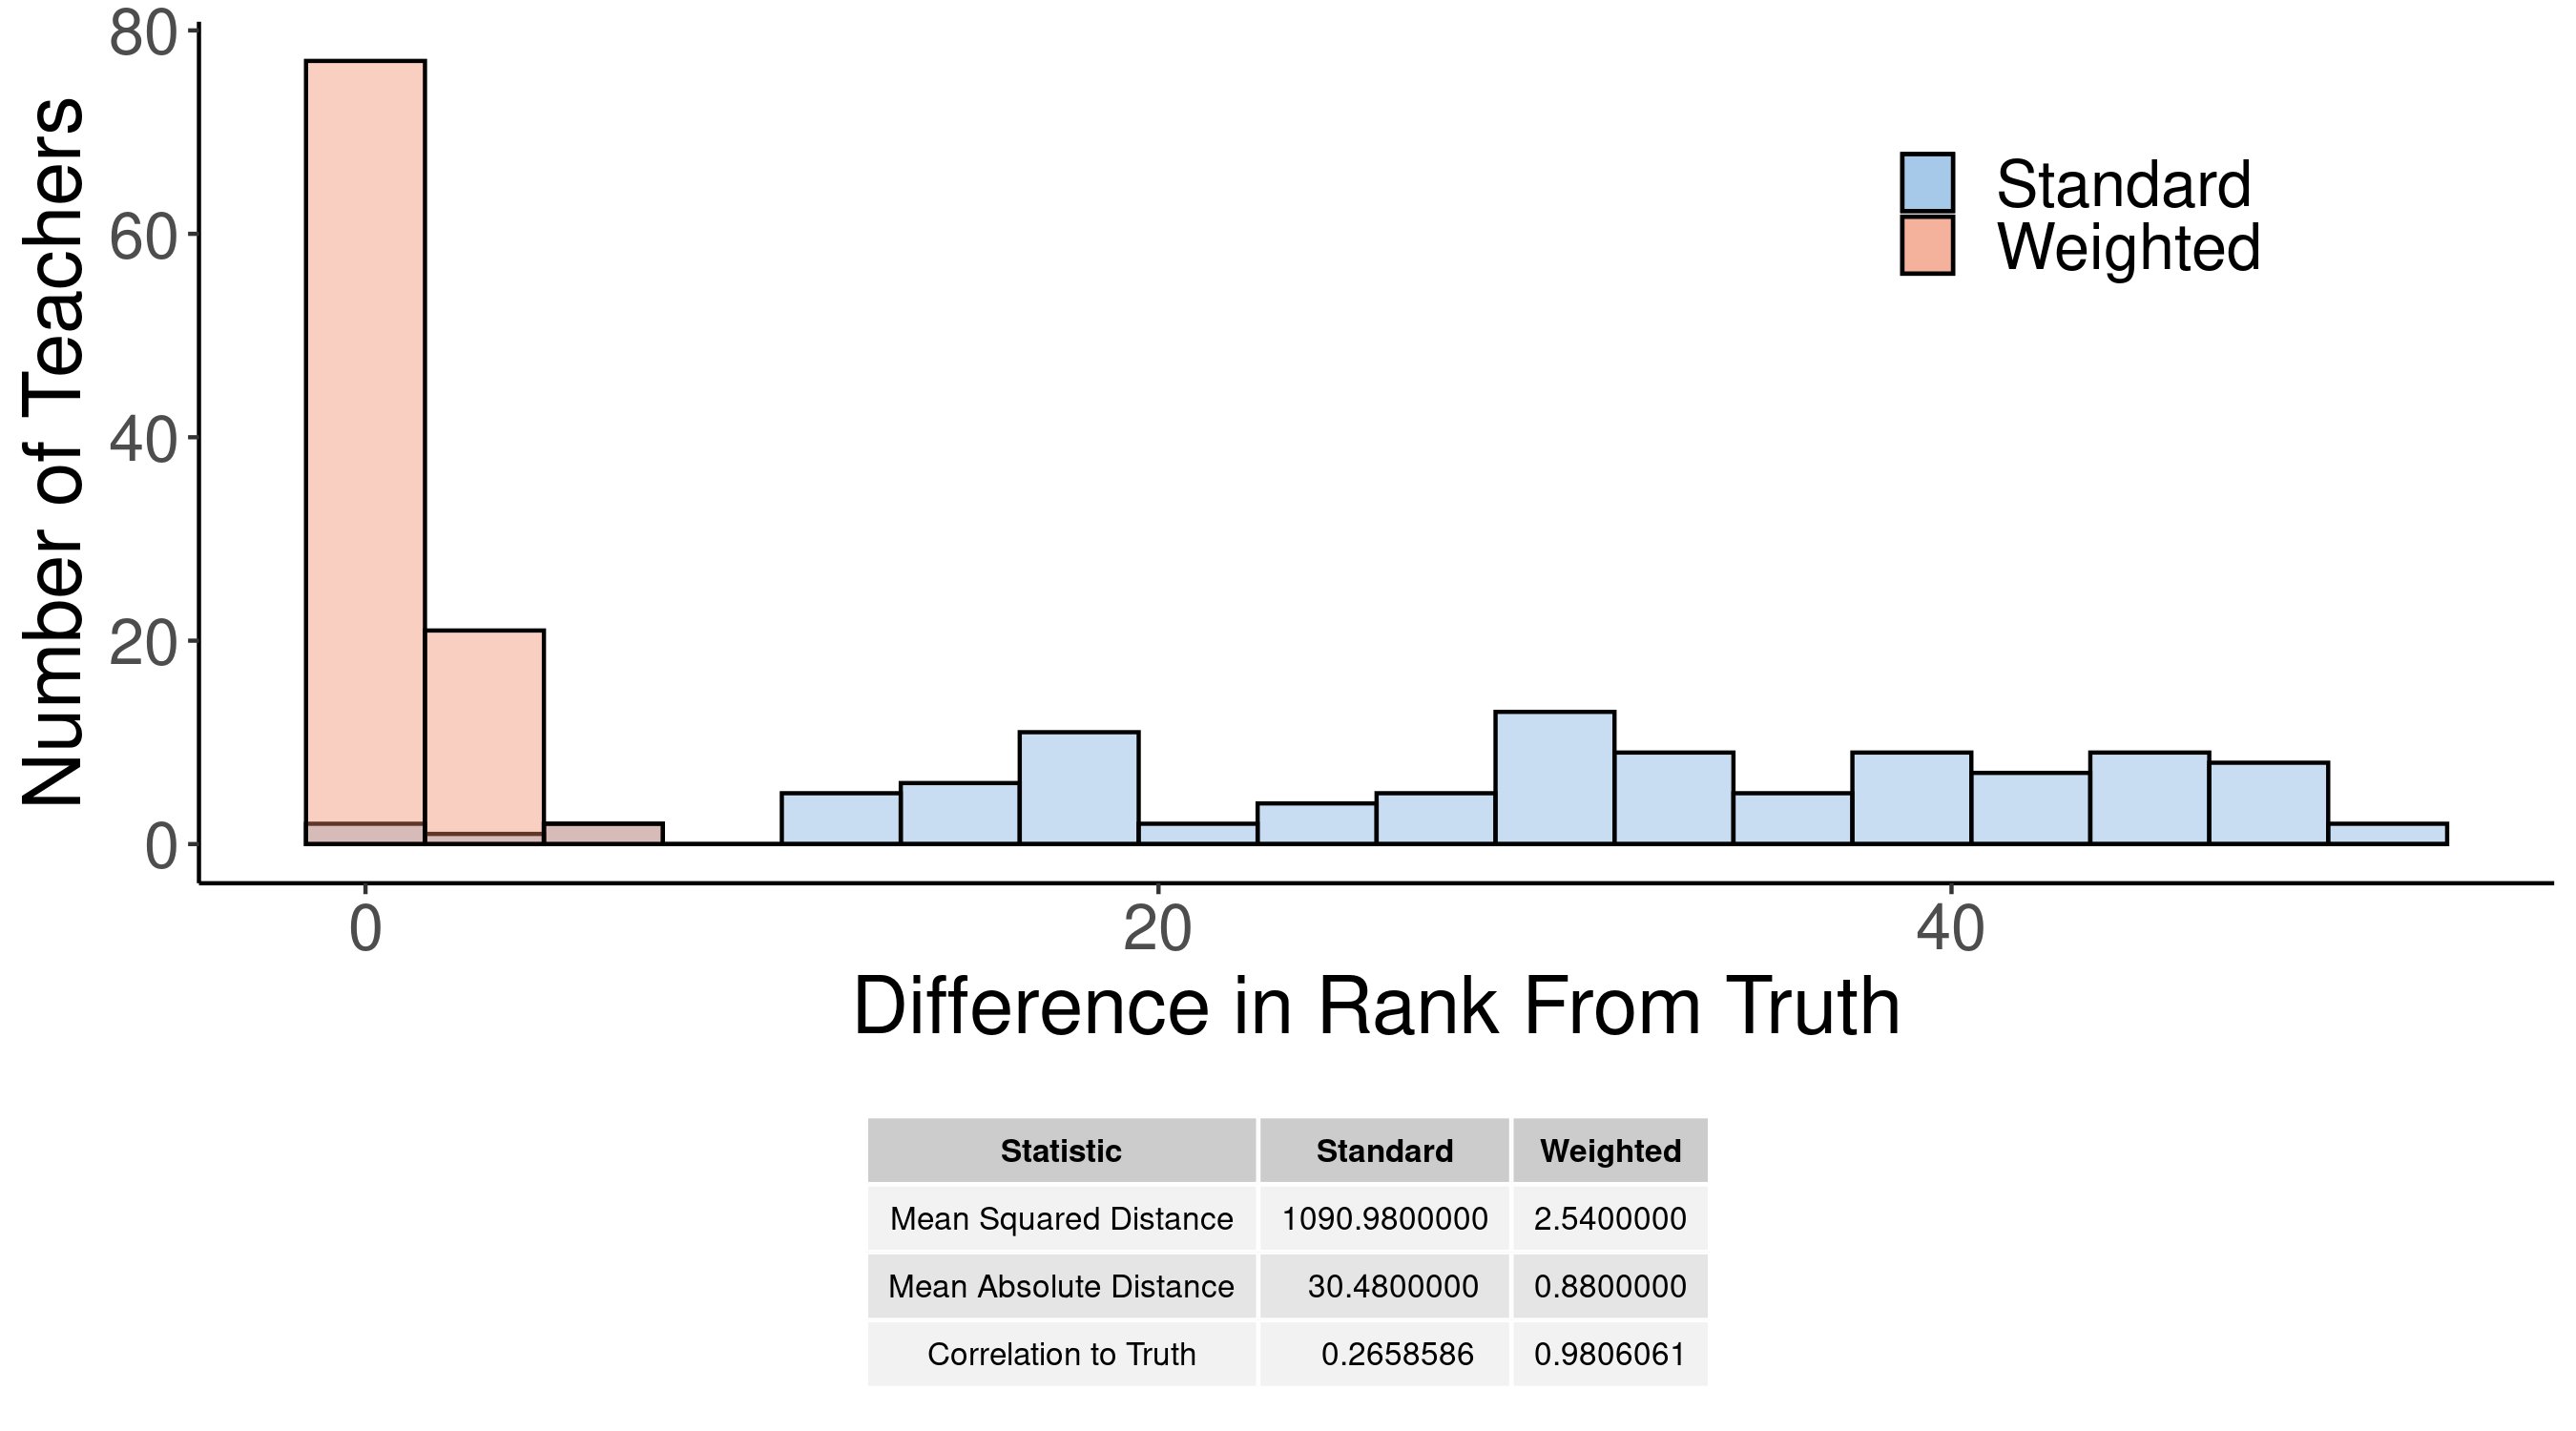
\includegraphics[width=\linewidth]{slides/Figures/hist_run_1.png}

\end{frame}


%%%%%%%%%%%%%%%%%%%%%%%%%%%%%%%%%%%%%%%%%%%%%%%%%%%%%%%%
%%%%%%%%%%%%%%%%%%%%%%%%%%%%%%%%%%%%%%%%%%%%%%%%%%%%%%%%

\begin{frame}{Results}

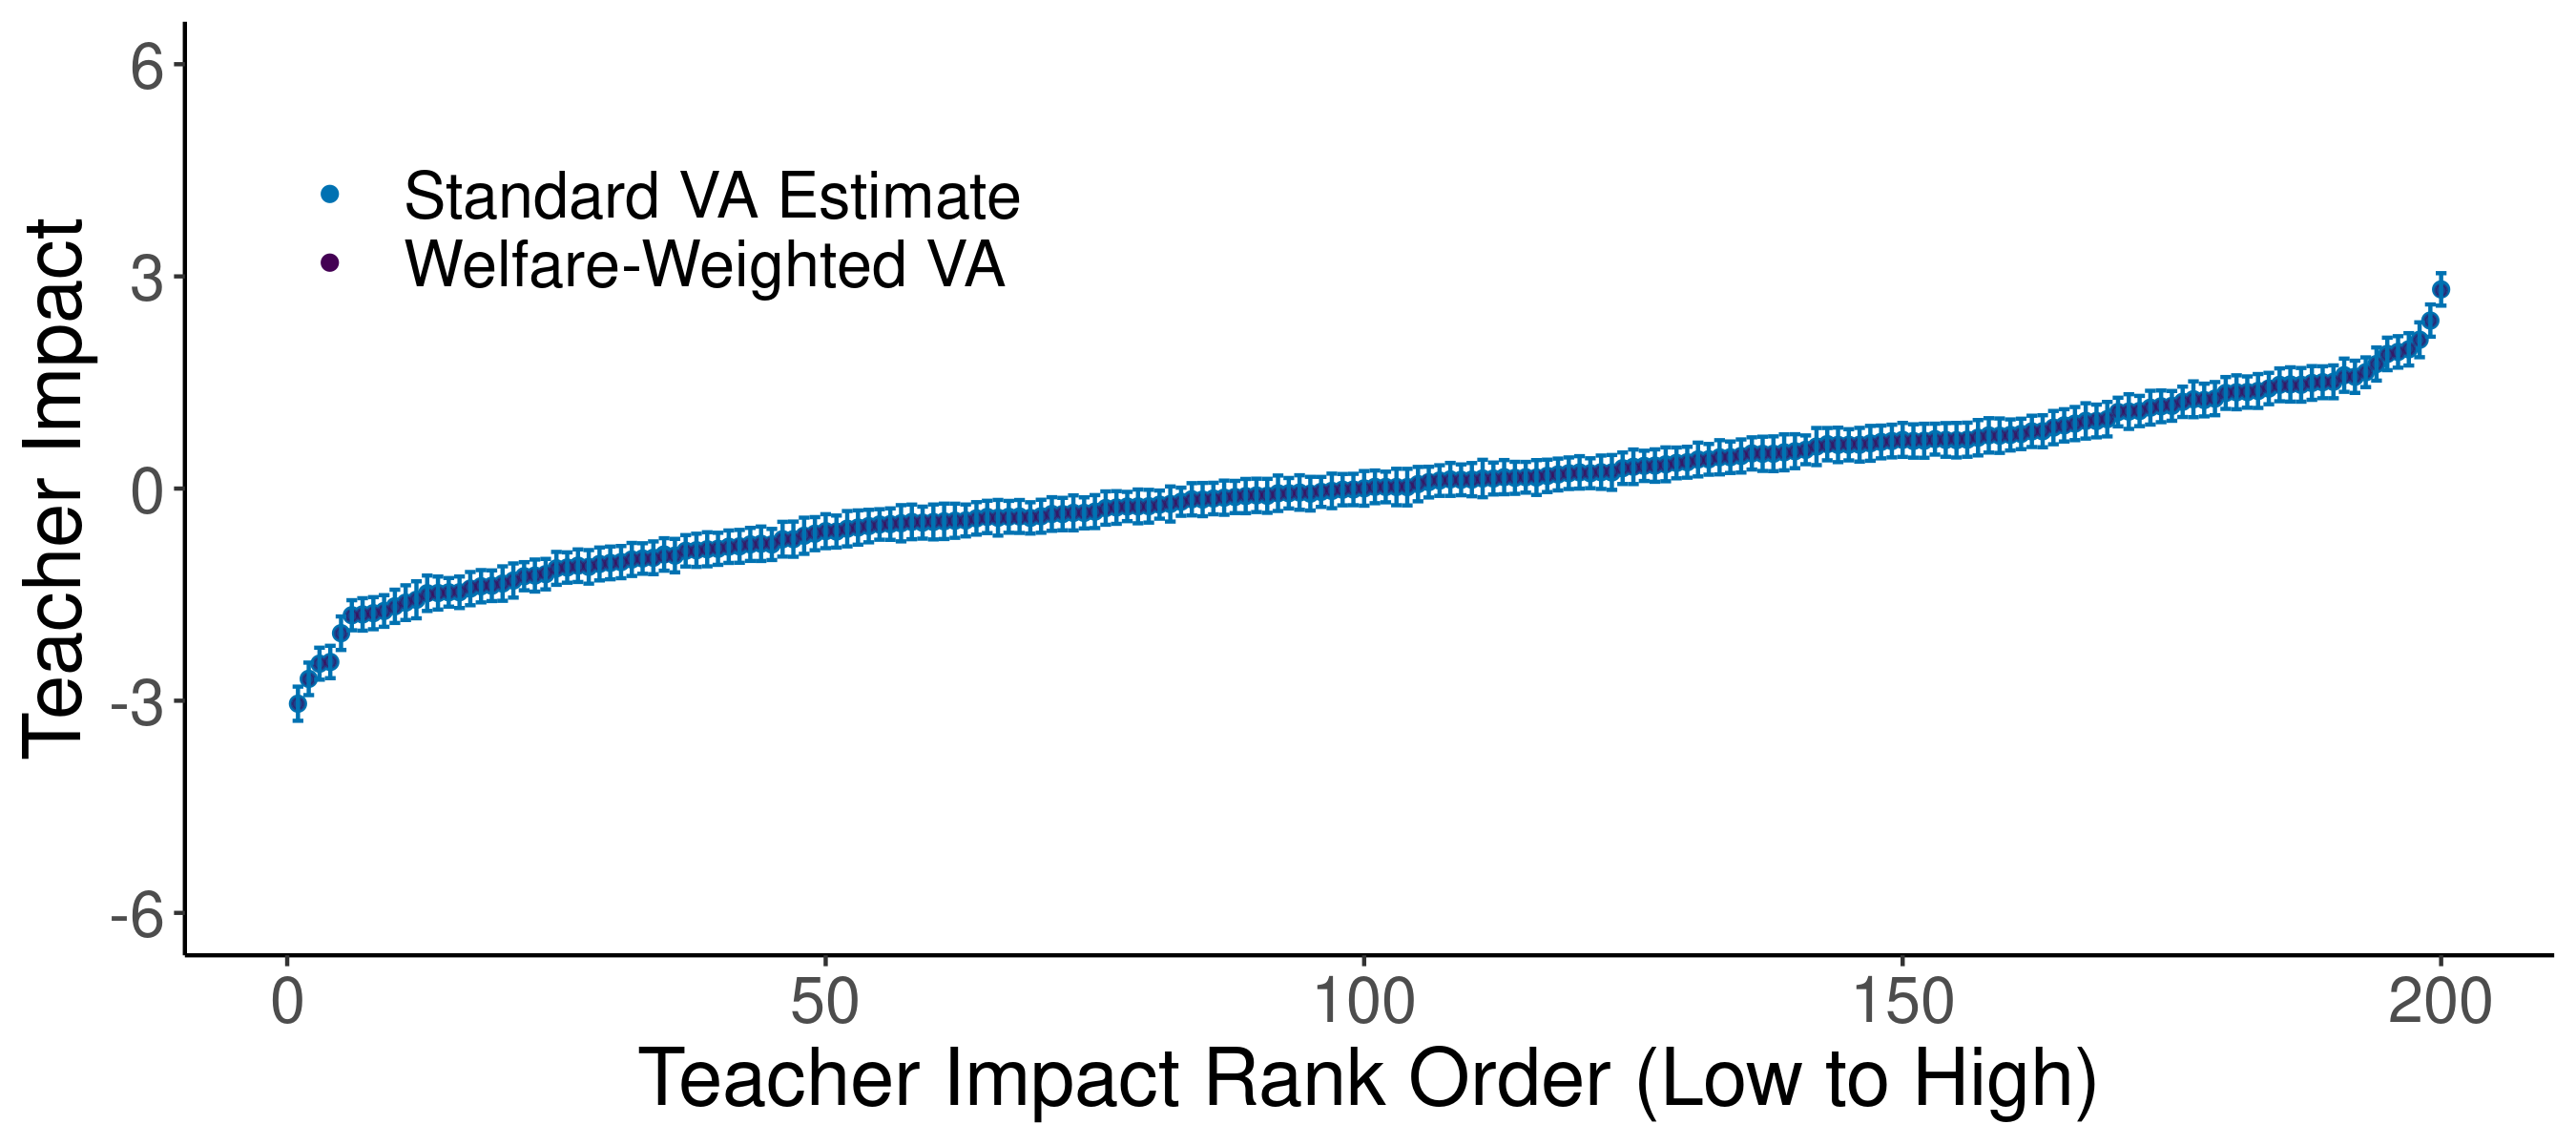
\includegraphics[width=\linewidth]{slides/Figures/standard_cat_run_1.png}

\end{frame}


%%%%%%%%%%%%%%%%%%%%%%%%%%%%%%%%%%%%%%%%%%%%%%%%%%%%%%%%
%%%%%%%%%%%%%%%%%%%%%%%%%%%%%%%%%%%%%%%%%%%%%%%%%%%%%%%%

\begin{frame}{Results}

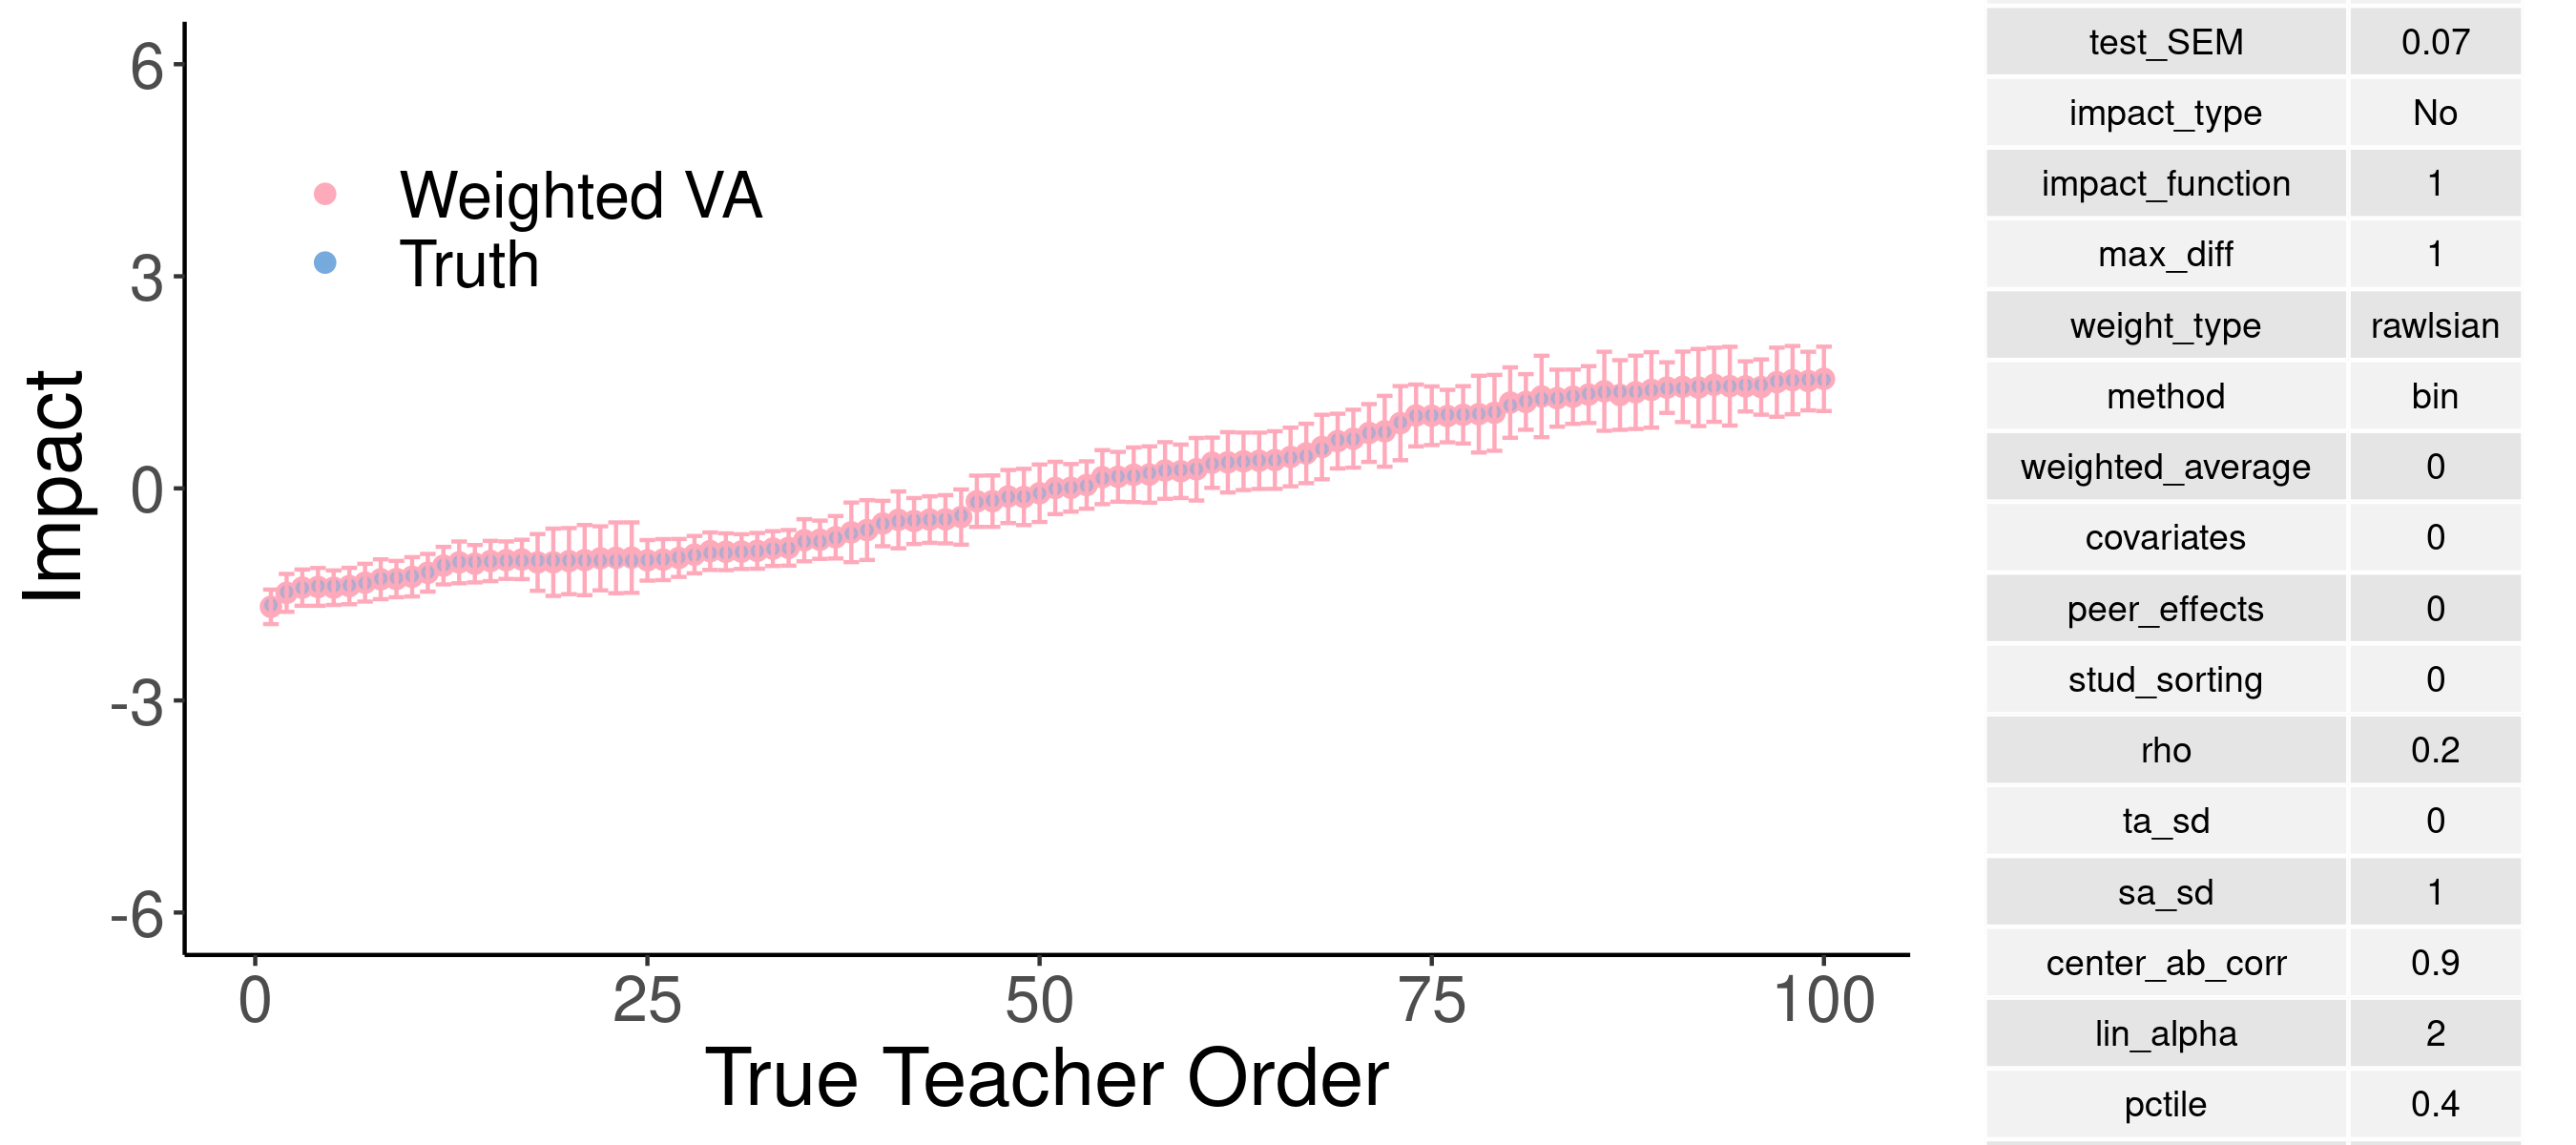
\includegraphics[width=\linewidth]{slides/Figures/ww_cat_run_1.png}

\end{frame}


%%%%%%%%%%%%%%%%%%%%%%%%%%%%%%%%%%%%%%%%%%%%%%%%%%%%%%%%
%%%%%%%%%%%%%%%%%%%%%%%%%%%%%%%%%%%%%%%%%%%%%%%%%%%%%%%%

\begin{frame}{Results}

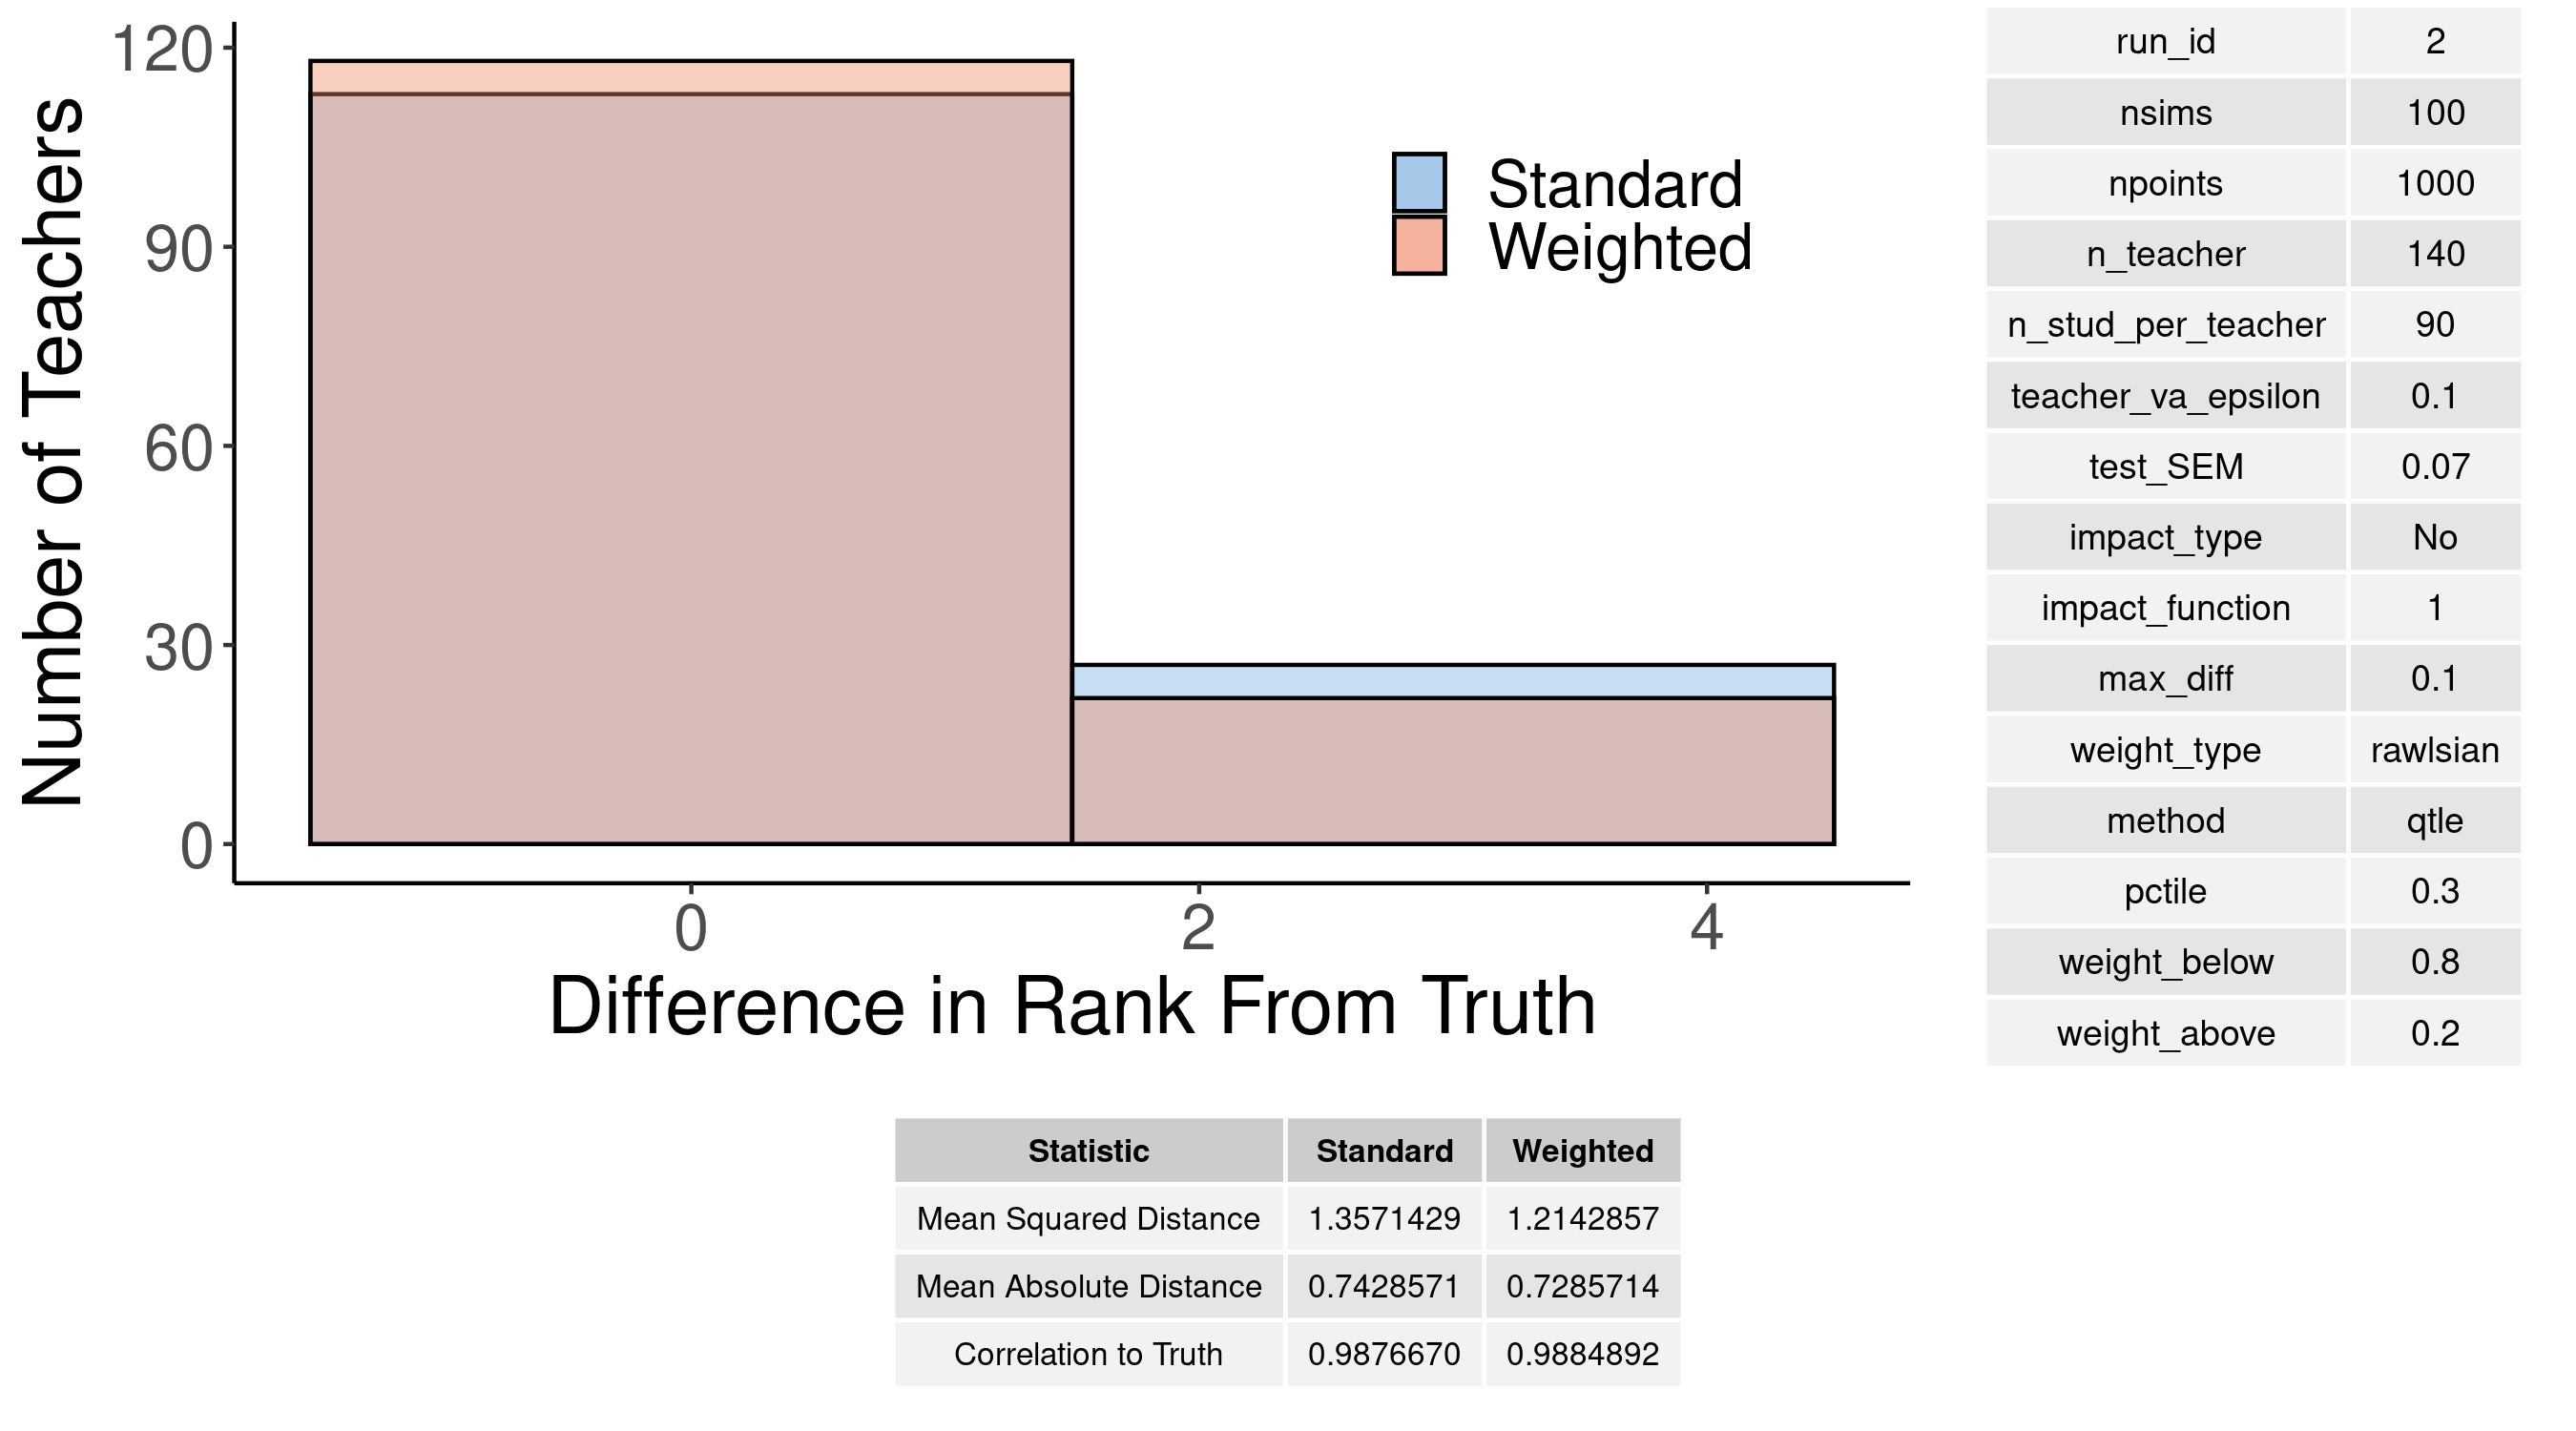
\includegraphics[width=\linewidth]{slides/Figures/hist_run_2.png}

\end{frame}


%%%%%%%%%%%%%%%%%%%%%%%%%%%%%%%%%%%%%%%%%%%%%%%%%%%%%%%%
%%%%%%%%%%%%%%%%%%%%%%%%%%%%%%%%%%%%%%%%%%%%%%%%%%%%%%%%

\begin{frame}{Results}

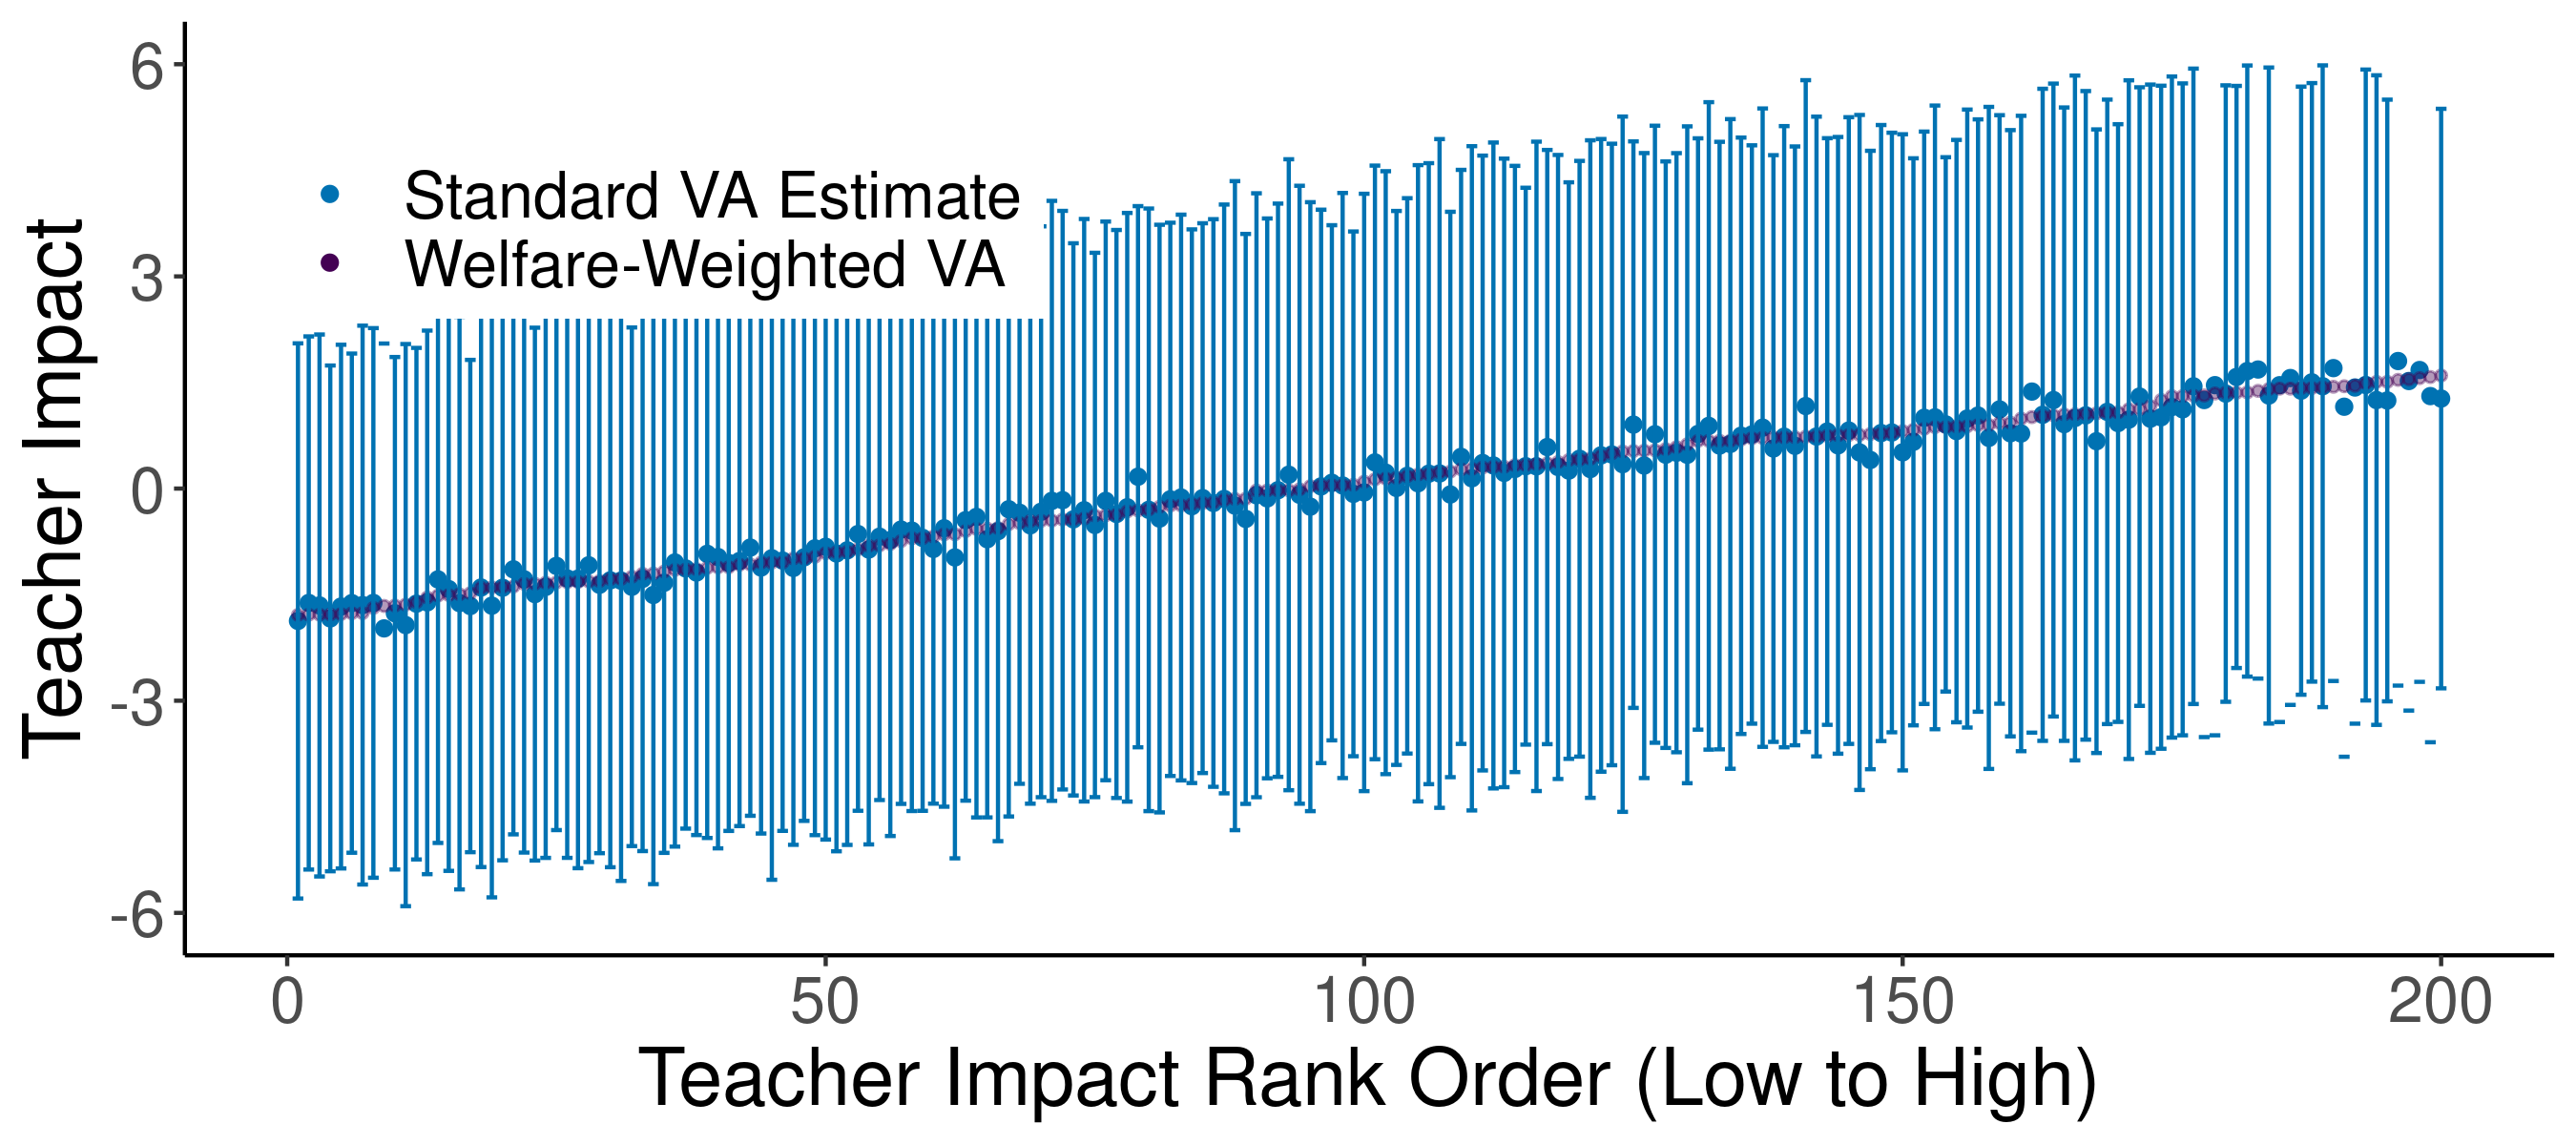
\includegraphics[width=\linewidth]{slides/Figures/standard_cat_run_2.png}

\end{frame}


%%%%%%%%%%%%%%%%%%%%%%%%%%%%%%%%%%%%%%%%%%%%%%%%%%%%%%%%
%%%%%%%%%%%%%%%%%%%%%%%%%%%%%%%%%%%%%%%%%%%%%%%%%%%%%%%%

\begin{frame}{Results}

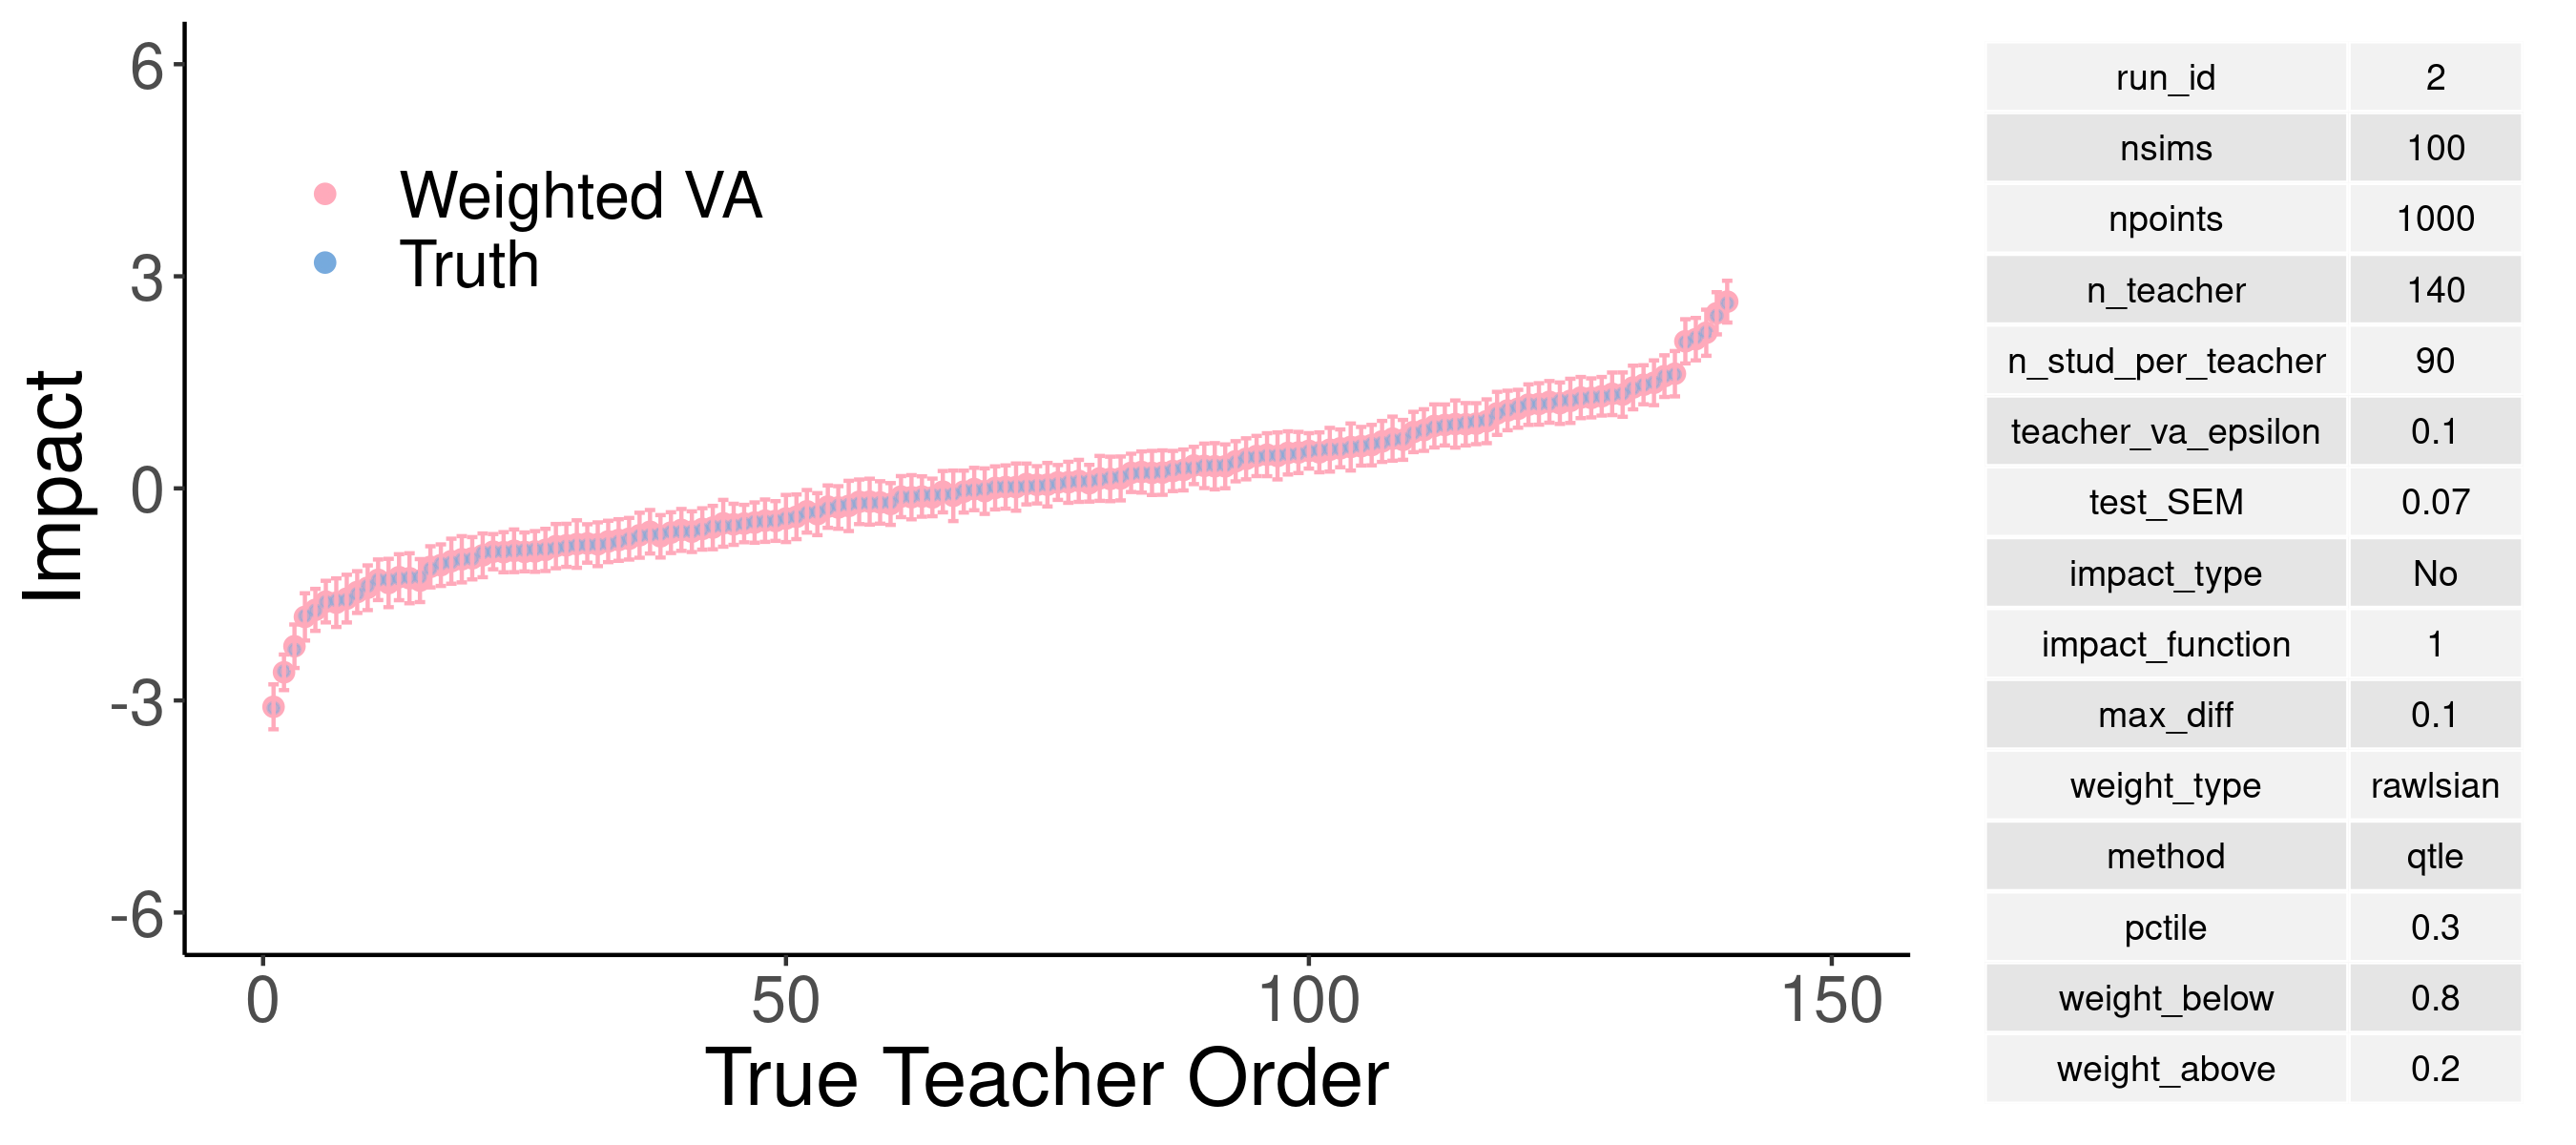
\includegraphics[width=\linewidth]{slides/Figures/ww_cat_run_2.png}

\end{frame}


%%%%%%%%%%%%%%%%%%%%%%%%%%%%%%%%%%%%%%%%%%%%%%%%%%%%%%%%
%%%%%%%%%%%%%%%%%%%%%%%%%%%%%%%%%%%%%%%%%%%%%%%%%%%%%%%%

\begin{frame}{}

\centering
\huge Thank you!

\end{frame}


%%%%%%%%%%%%%%%%%%%%%%%%%%%%%%%%%%%%%%%%%%%%%%%%%%%%%%%%
%%%%%%%%%%%%%%%%%%%%%% References %%%%%%%%%%%%%%%%%%%%%%
%%%%%%%%%%%%%%%%%%%%%%%%%%%%%%%%%%%%%%%%%%%%%%%%%%%%%%%%

\section*{}
\begin{frame}[noframenumbering, shrink=10]
    \frametitle{References}
    \bibliography{citations}
\end{frame}


\end{document}
